\section{Part 1: MDPs and Reinforcement Learning}
For parts 1.1 and 1.2, we provide a video of the run with animated simulation to show that we are able to reach the goal and the policies are acceptable. The video can be found here: https://youtu.be/vgN8rnYWBgU.

For the extra credit for parts 1.1 and 1.2, we also provide such a video here: https://youtu.be/7eJJ0lHUO5U

\subsection{Part 1.1: Grid World MDP}
%% \begin{itemize}
%%   \item \Fix{Discuss implement of value OR policy iteration.}
%%   \item \Fix{Show the optimal policy and utilities of all states for terminal AND non-terminal reward squares scenarios.}
%%   \item \Fix{Plot utility estimates as a function of the number of iterations.}
%% \end{itemize}

We implemented value iteration with 50 iterations with the following parameter settings:
\begin{itemize}
  \item Learning rate decay function ($\alpha$): $\frac{100}{99+t}$, where $t$ is the number of iterations.
  \item Discount factor ($\gamma$): 0.99
\end{itemize}

In our value iteration implementation, we created 2D arrays to keep track of utilities and policies for each coordinate on the map. Each coordinate is associated with one utility value and one policy (direction) at any given iteration/time. For example, we create the data structure utility\_ ra[height][width] to hold the utility at coordinate (height, width).

\subsubsection{a: Terminal rewards}
\begin{figure}[H]
  \centering
  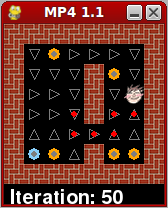
\includegraphics[width=0.2\linewidth]{graphics/term_11_opti_policy.png}
  \caption{Terminal rewards: optimal policy}
\end{figure}

\paragraph{Left half of utilities}
\begin{tabular}{|l|l|l|l|}
0 & 0 & 0 & 0 \\
0 & 1.6663819929603512 & -1.0 & 1.8122075850456765 \\
0 & 2.0712250112362023 & 2.140515760142894 & 2.2100465635812827 \\
0 & 2.139220576435563 & 2.218017533372307 & 2.2971476009987657 \\
0 & 2.196963903424736 & 2.290561404847123 & 2.3865483022244462 \\
0 & 2.1318832563135315 & 2.230620373624008 & 2.4791849017833654 \\
0 & 1.0 & -1.0 & 2.024988281755731 \\
0 & 0 & 0 & 0 \\
\end{tabular}

\paragraph{Right half of utilities}
\begin{tabular}{|l|l|l|l|}
0 & 0 & 0 & 0 \\
1.8358641737026038 & 1.90954932741097 & 2.347858515148086 & 0 \\
0 & -1.0 & 2.4827968923418426 & 0 \\
0 & 2.743906705960116 & 3.0 & 0 \\
0 & 2.797045381404416 & 2.9000083160474563 & 0 \\
2.629346944690836 & 2.7130508202637618 & 2.802884148184854 & 0 \\
0 & -1.0 & -1.0 & 0 \\
0 & 0 & 0 & 0 \\
\end{tabular}

\begin{figure}[H]
  \centering
  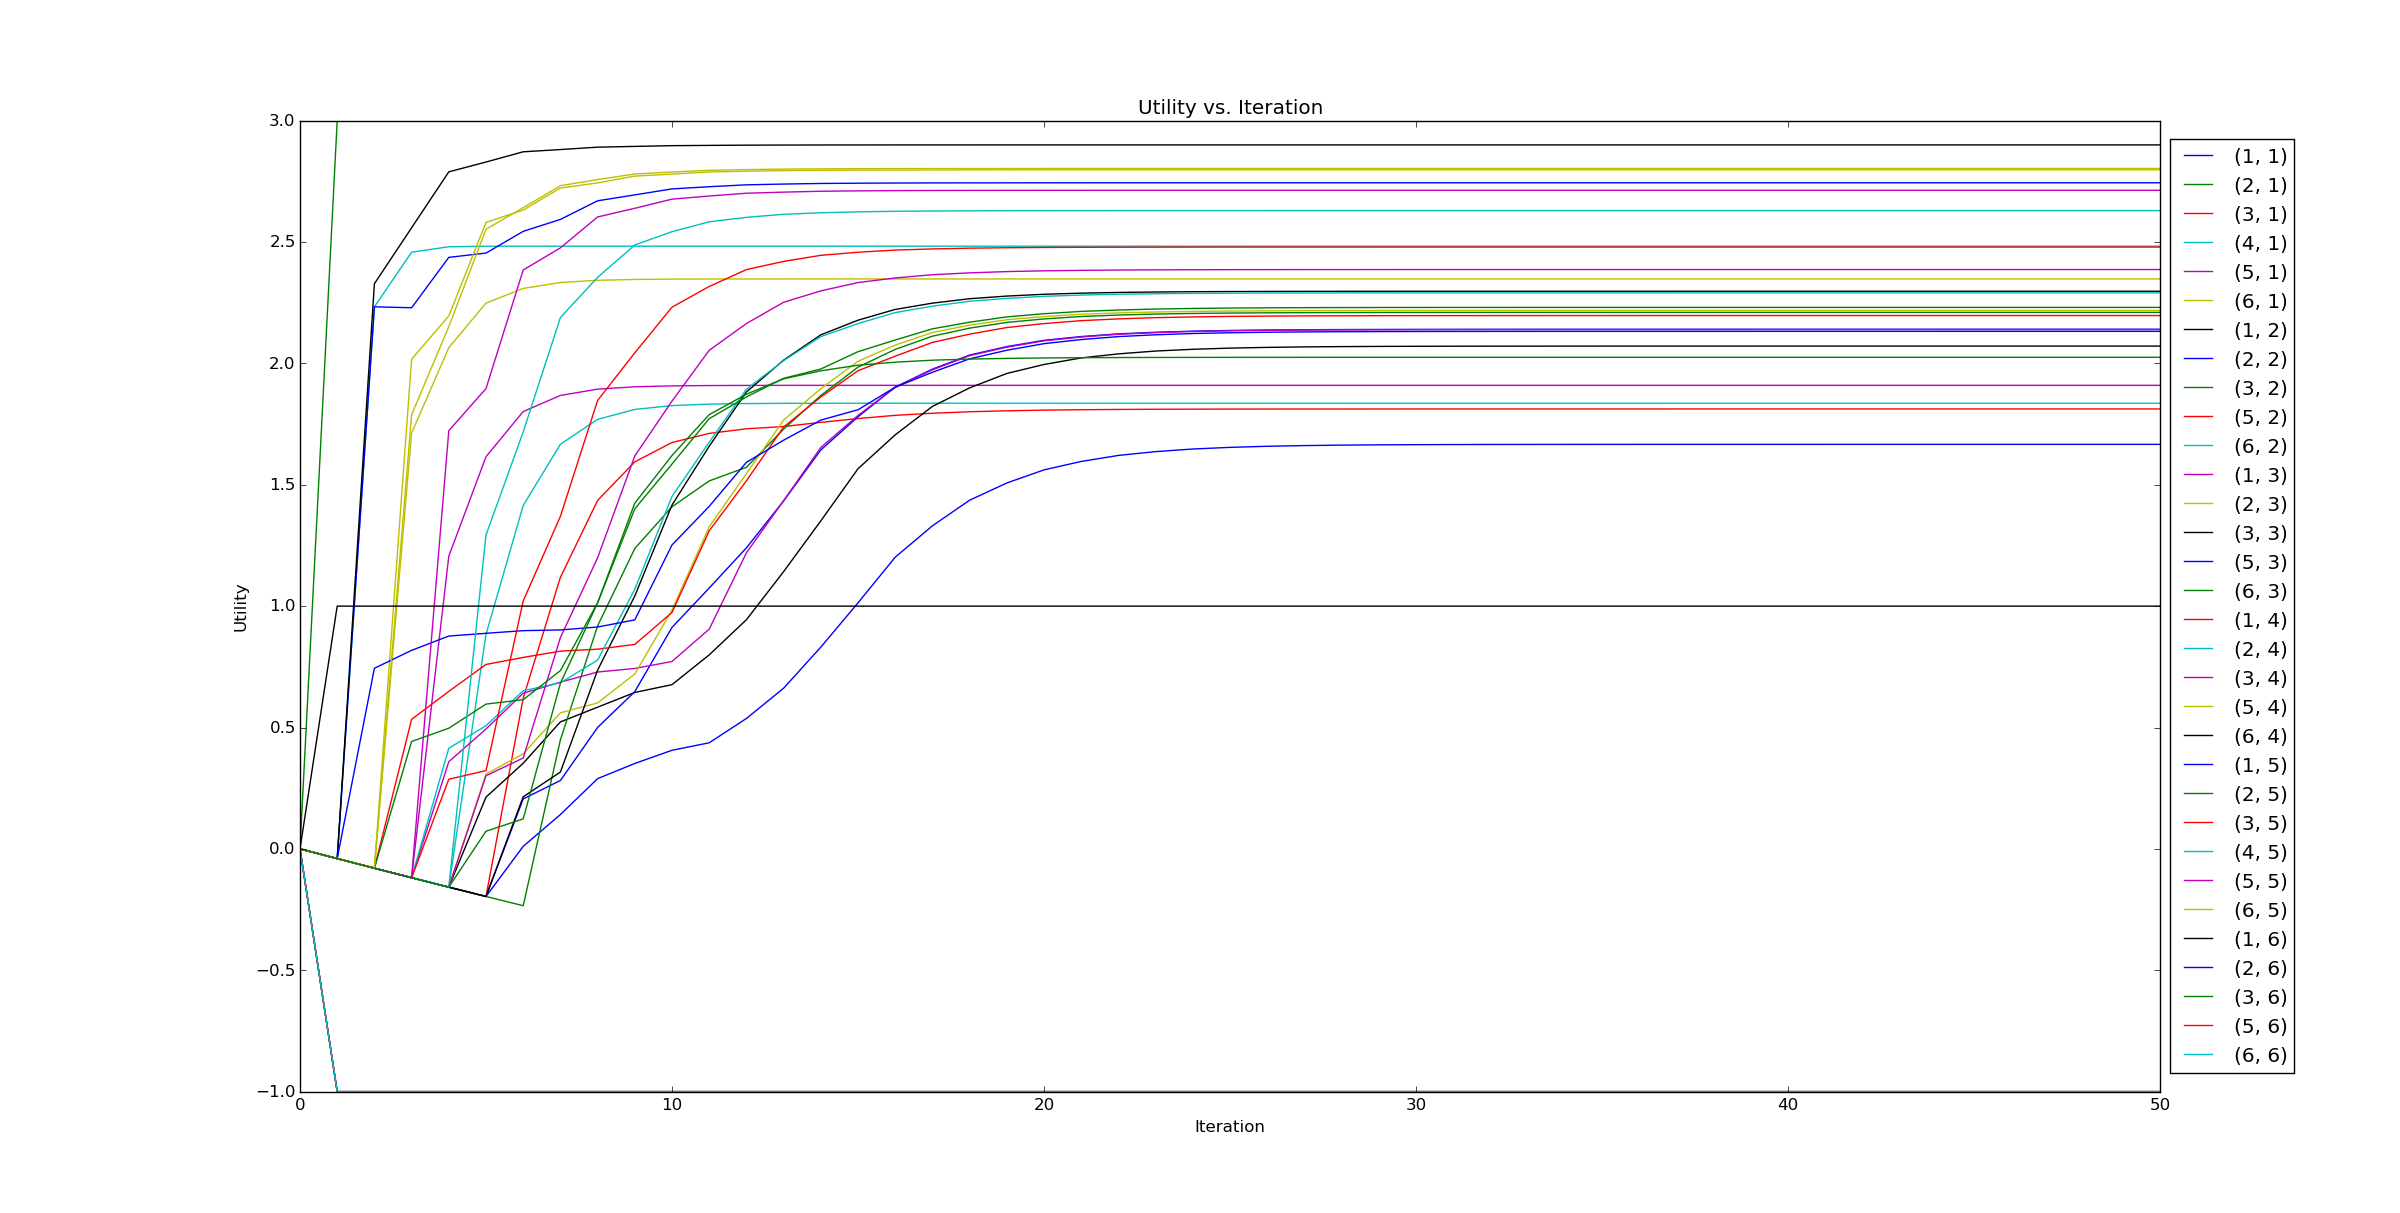
\includegraphics[width=\linewidth]{graphics/term_11_util_iters.png}
  \caption{Terminal rewards: utility estimates vs number of iterations}
\end{figure}

\subsubsection{b: Non-terminal rewards}
\begin{figure}[H]
  \centering
  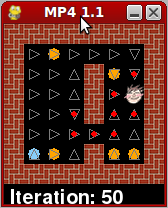
\includegraphics[width=0.2\linewidth]{graphics/inf_11_opti_policy.png}
  \caption{Non-terminal rewards: optimal policy (end state policy arrow is towards the right)}
\end{figure}

\paragraph{Left half of utilities}
\begin{tabular}{|l|l|l|l|}
0 & 0 & 0 & 0 \\
0 & 70.15796135830524 & 73.06273393250066 & 77.23882007176084 \\
0 & 68.60441398357725 & 71.32905910580921 & 74.12821672939297 \\
0 & 66.78141487176684 & 69.00504921113657 & 71.13856653329579 \\
0 & 68.51290895967463 & 71.18107818479461 & 73.88353477498987 \\
0 & 70.41751555235511 & 73.52543278791883 & 76.97896106942257 \\
0 & 69.16963507078813 & 70.26634298614438 & 73.78302558002932 \\
0 & 0 & 0 & 0 \\
\end{tabular}
\paragraph{Right half of utilities}
\begin{tabular}{|l|l|l|l|}
0 & 0 & 0 & 0 \\
80.42762942372242 & 83.26787610223616 & 85.89848178463846 & 0 \\
0 & 85.23189767501776 & 89.13663059215091 & 0 \\
0 & 88.85683390367892 & 92.57493102127128 & 0 \\
0 & 86.31040141566613 & 89.25513433279929 & 0 \\
80.56208417850117 & 83.40402851806007 & 86.01760947804587 & 0 \\
0 & 79.62059497140713 & 81.69055109171586 & 0 \\
0 & 0 & 0 & 0 \\
\end{tabular}

\paragraph{}
\begin{figure}[H]
  \centering
  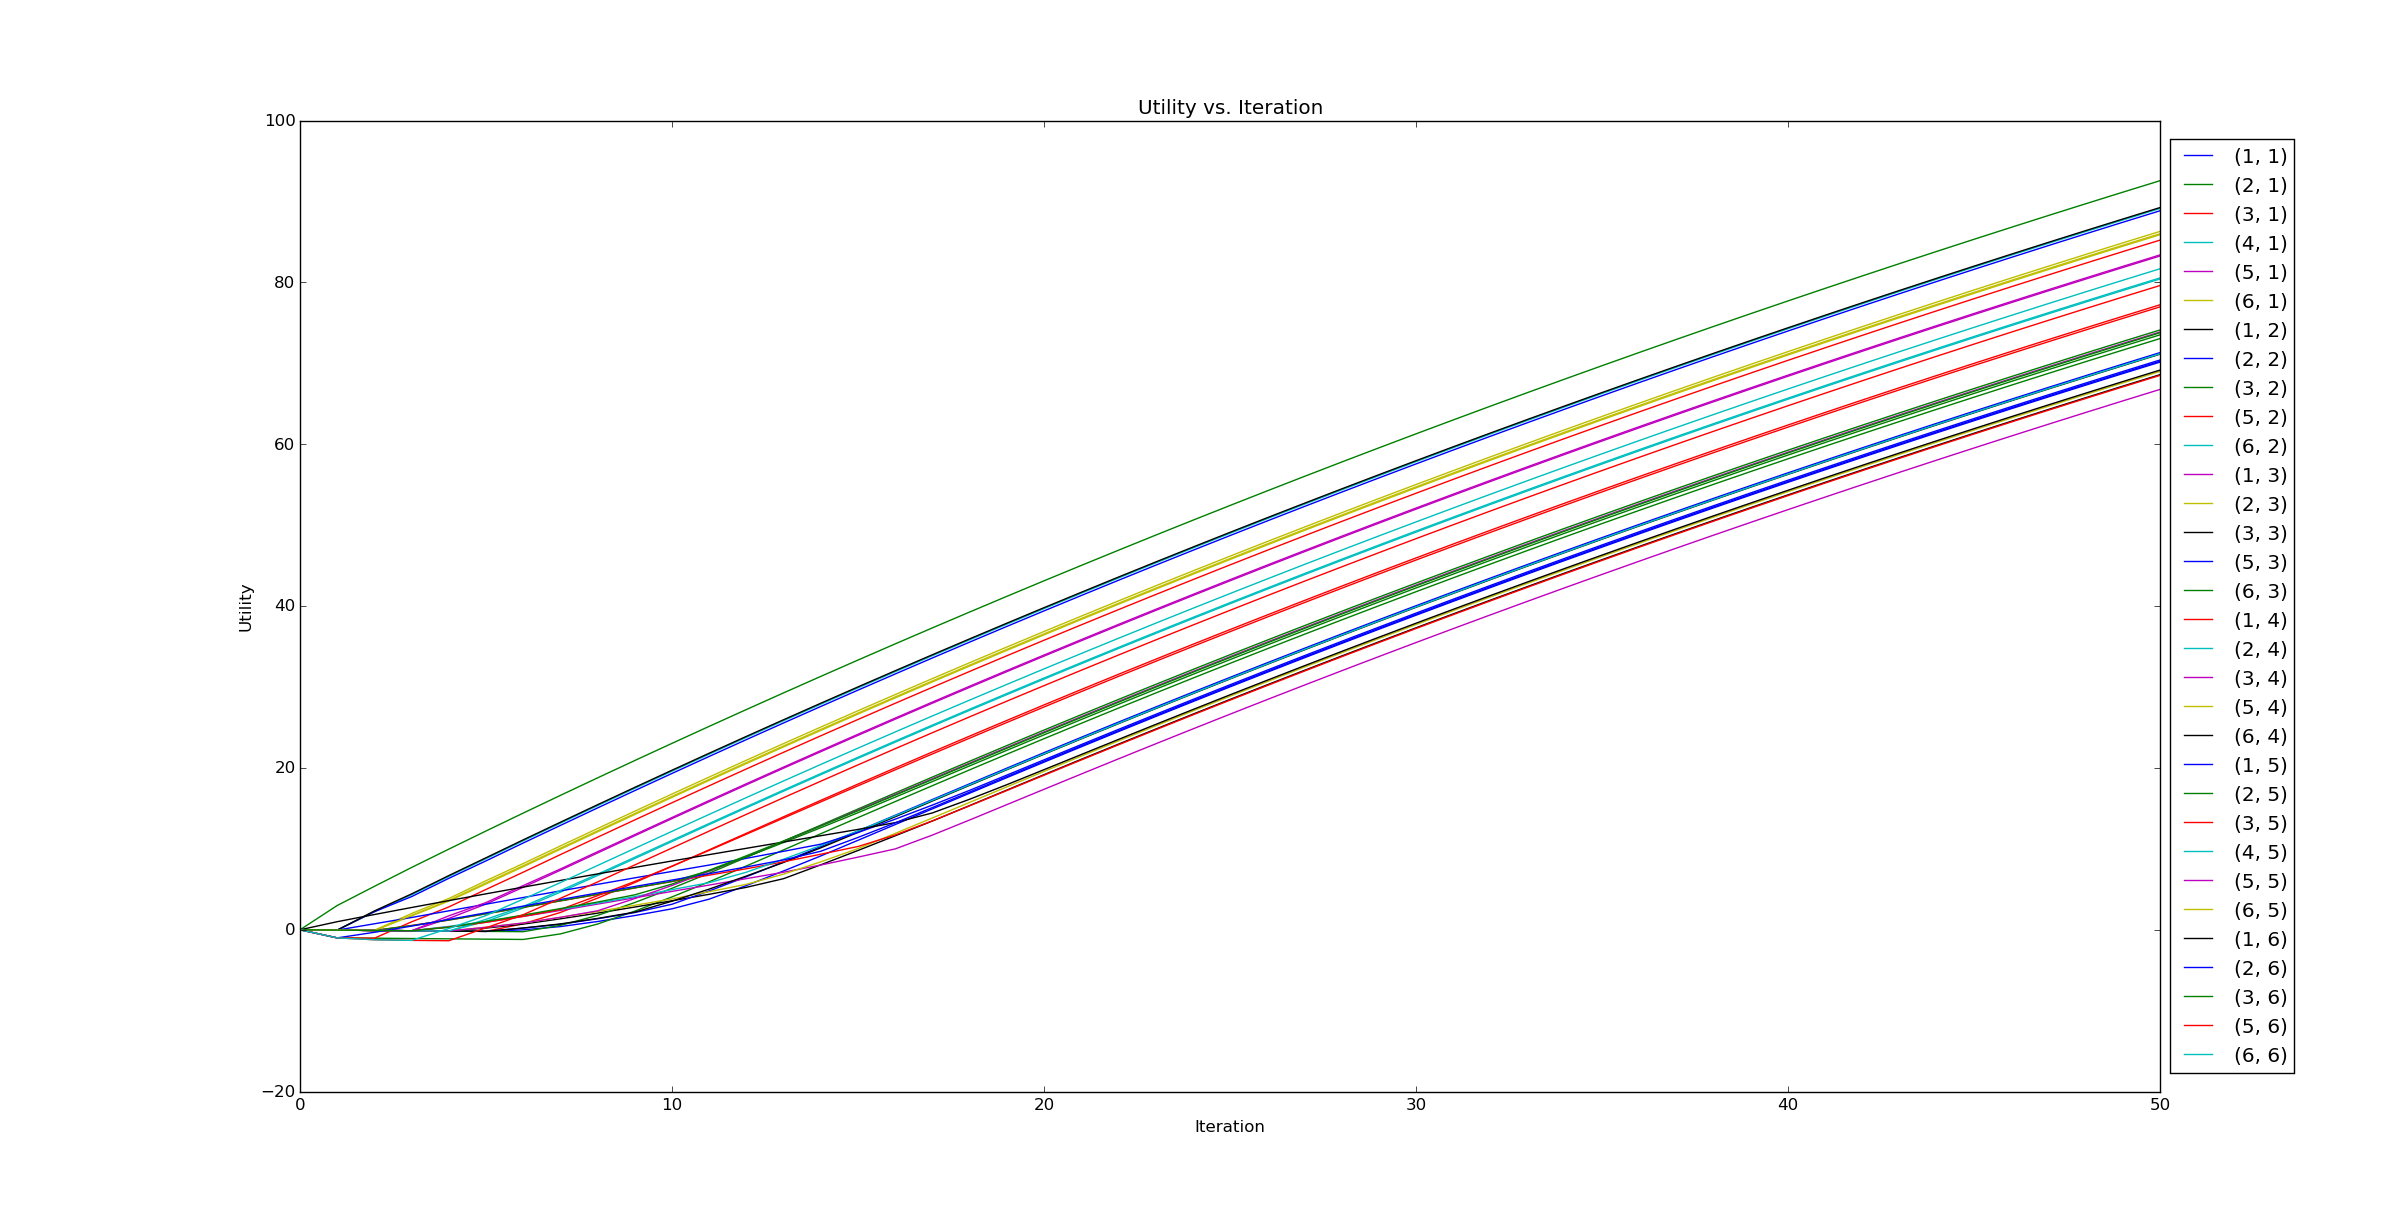
\includegraphics[width=1\linewidth]{graphics/inf_11_util_iters.png}
  \caption{Terminal rewards: utility estimates vs \# of iterations}
\end{figure}


\subsection{Part 1.2: Grid World Reinforcement Learning}
%% \begin{itemize}
%%   \item \Fix{Discuss implementation of TD Q-learning and parameter settings.}
%%   \item \Fix{Give utility estimates.}
%%   \item \Fix{Plot RMS error as a function of the number of trials.}
%% \end{itemize}

We implemented TD Q-learning with the following parameters:
\begin{itemize}
  \item Learning rate decay function ($\alpha$): $\frac{100}{99+t}$, where $t$ is the number of iterations.
  \item Discount factor ($\gamma$): 0.99
  \item Exploration function: if the number of visited places is less than 100 or if an action at a state was repeated, then try a random action. Otherwise, follow the standard exploration function on slide 21 of lecture 17 (Reinforcement learning).
\end{itemize}

In our TD Q-learning implementation, each coordinate in the map has a single policy (direction) and four utilities associated with it, one for each direction that the pacman could (possibly) move in for its action. We created the data structures utility\_ ra = max{value[height][width]} to hold the utility at each coordinate and value\_ ra[height][width][action] to hold the four values for the four directions at each coordinate, just as slide 22 of lecture 17 (Reinforcement learning) shows. At some coordinate (height, width), the maximum of the four values in the value\_ ra at that coordinate is the utility at that coordinate.

%% Final RMS Error: 0.0280277380717

\subsubsection{Utility estimates}
\paragraph{Left half of utilities}
\begin{tabular}{|l|l|l|l|}
0 & 0 & 0 & 0 \\
0 & 1.5771197238920487 & -1.0 & 1.8621867629158122 \\
0 & 2.060156352764028 & 2.131697265185684 & 2.2078804206262648 \\
0 & 2.1294033483030246 & 2.2090285226278548 & 2.276761045134516 \\
0 & 2.187062025112003 & 2.284226513177173 & 2.3692453367427873 \\
0 & 2.1243000485531875 & 2.2181717049601577 & 2.4779495615664118 \\
0 & 1.0 & -1.0 & 1.9755292527709516 \\
0 & 0 & 0 & 0 \\
\end{tabular}

\paragraph{Right half of utilities}
\begin{tabular}{|l|l|l|l|}
0 & 0 & 0 & 0 \\
1.8123661183379303 & 1.8048504083978827 & 2.284447718223661 & 0 \\
0 & -1.0 & 2.3409971810811316 & 0 \\
0 & 2.741332171514045 & 3.0 & 0 \\
0 & 2.7920529231276925 & 2.9047606396921575 & 0 \\
2.6156932575513423 & 2.70937566453376 & 2.807136539903526 & 0 \\
0 & -1.0 & -1.0 & 0 \\
0 & 0 & 0 & 0 \\
\end{tabular}

\subsubsection{RMS error versus number of trials}
\begin{figure}[H]
  \centering
  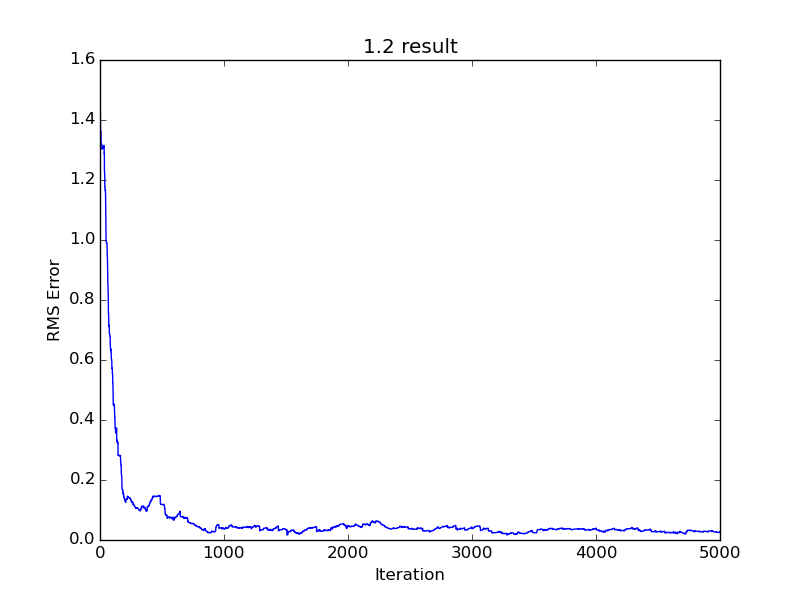
\includegraphics[width=0.5\linewidth]{graphics/rmse_plot_12.png}
  \caption{RMS error vs number of iterations}
\end{figure}

\newpage
\subsection{Extra credit: 1.1 and 1.2}
We created a more complicated environment of width 23 and height 8 (Red: -3, Yellow: -1, Sky Blue: +1, Blue: +3), and show the same data as for 1.1 and 1.2, except for the final utilities matrix, which is too large to display.

Additionally, matplotlib did not have enough colors to represent all of the states, so the utility estimates plot shows utility estimates with repeated colors but gives the general idea of how the states' utilities changed.

Due to the higher number of states, we needed about 200 iterations to start converging, compared to 50 iterations for the smaller 8x8 environment.

\subsubsection{Terminal rewards value iteration}
\begin{figure}[H]
  \centering
  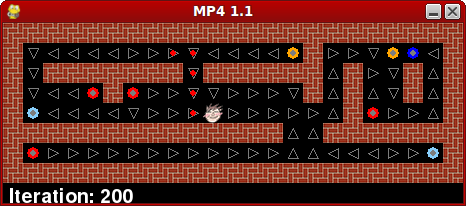
\includegraphics[width=0.5\linewidth]{graphics/term_11ec_opti_policy.png}
  \caption{Terminal rewards: optimal policy (ended on a +1 reward state)}
\end{figure}

%% \paragraph{Utilities}
%% \begin{tabular}{|l|l|l|l|l|l|l|l|l|l|l|l|l|l|l|l|l|l|l|l|l|l|l|}
%% 0 & 0 & 0 & 0 & 0 & 0 & 0 & 0 & 0 & 0 & 0 & 0 & 0 & 0 & 0 & 0 & 0 & 0 & 0 & 0 & 0 & 0 & 0 \\
%% 0 & 0.8013117744290585 & 0.7414450440745814 & 0.6823247816796365 & 0.623941679663681 & 0.566286546500792 & 0.5592995527031022 & 0.6168664662473333 & 0.6751602347605573 & 0.7341900357045039 & 0.6751602347605573 & 0.6168664662473333 & 0.5592995527031022 & 0.5024504310983253 & -1.0 & 0 & 1.5461633735735012 & 1.6248349584936144 & 1.6958556019089377 & -1.0 & 3.0 & 2.9020947105996022 & 0 \\
%% 0 & 0.8694177391378766 & 0 & 0 & 0 & 0 & 0 & 0 & 0 & 0.8087226126539314 & 0 & 0 & 0 & 0 & 0 & 0 & 1.477009216795777 & 0 & 2.1136325012854416 & 2.2483632902829793 & 0 & 2.816033679295368 & 0 \\
%% 0 & 0.9309002863492134 & 0.8761733131377903 & 0.8207235617464977 & -3.0 & 0 & -3.0 & 0.7593276176268648 & 0.814659086237458 & 0.8694388072581476 & 0.9303089889662338 & 0.9316620913906787 & 0.9894892975161349 & 1.0468802550296894 & 1.103523131068182 & 0 & 1.40871733129957 & 0 & 2.07110172517512 & 2.344098114795083 & 0 & 2.7310457281819596 & 0 \\
%% 0 & 1.0 & 0.9309002863492134 & 0.8640673245299448 & 0.38550646063009586 & 0.3308243351858304 & 0.3446913286785366 & 0.7974160321387719 & 0.862750518701987 & 0.9301603128951793 & 1.0 & 0.9671921283860878 & 1.0343504553386211 & 1.103523131068182 & 1.1750419139450663 & 1.2563948488371932 & 1.3319502956982703 & 0 & -3.0 & 2.4583249124217588 & 2.554147768595065 & 2.6369021596126787 & 0 \\
%% 0 & 0 & 0 & 0 & 0 & 0 & 0 & 0 & 0 & 0 & 0 & 0 & 0 & 0 & 1.118468724144033 & 1.1829002485785973 & 0 & 0 & 0 & 0 & 0 & 0 & 0 \\
%% 0 & -3.0 & 0.3468325407715976 & 0.4017167900237641 & 0.4572940222210338 & 0.5135729871480671 & 0.5705625450666034 & 0.6282716681103737 & 0.6867094416976258 & 0.7458850659614847 & 0.8058078571983721 & 0.8664872493347153 & 0.9279327954121739 & 0.9901541690916205 & 1.0531611661761107 & 1.1041280193329923 & 1.0404855253263465 & 0.9776365786265169 & 0.91557128462868 & 0.8760890790480158 & 0.9376558603491272 & 1.0 & 0 \\
%% 0 & 0 & 0 & 0 & 0 & 0 & 0 & 0 & 0 & 0 & 0 & 0 & 0 & 0 & 0 & 0 & 0 & 0 & 0 & 0 & 0 & 0 & 0 \\
%% \end{tabular}

\begin{figure}[H]
  \centering
  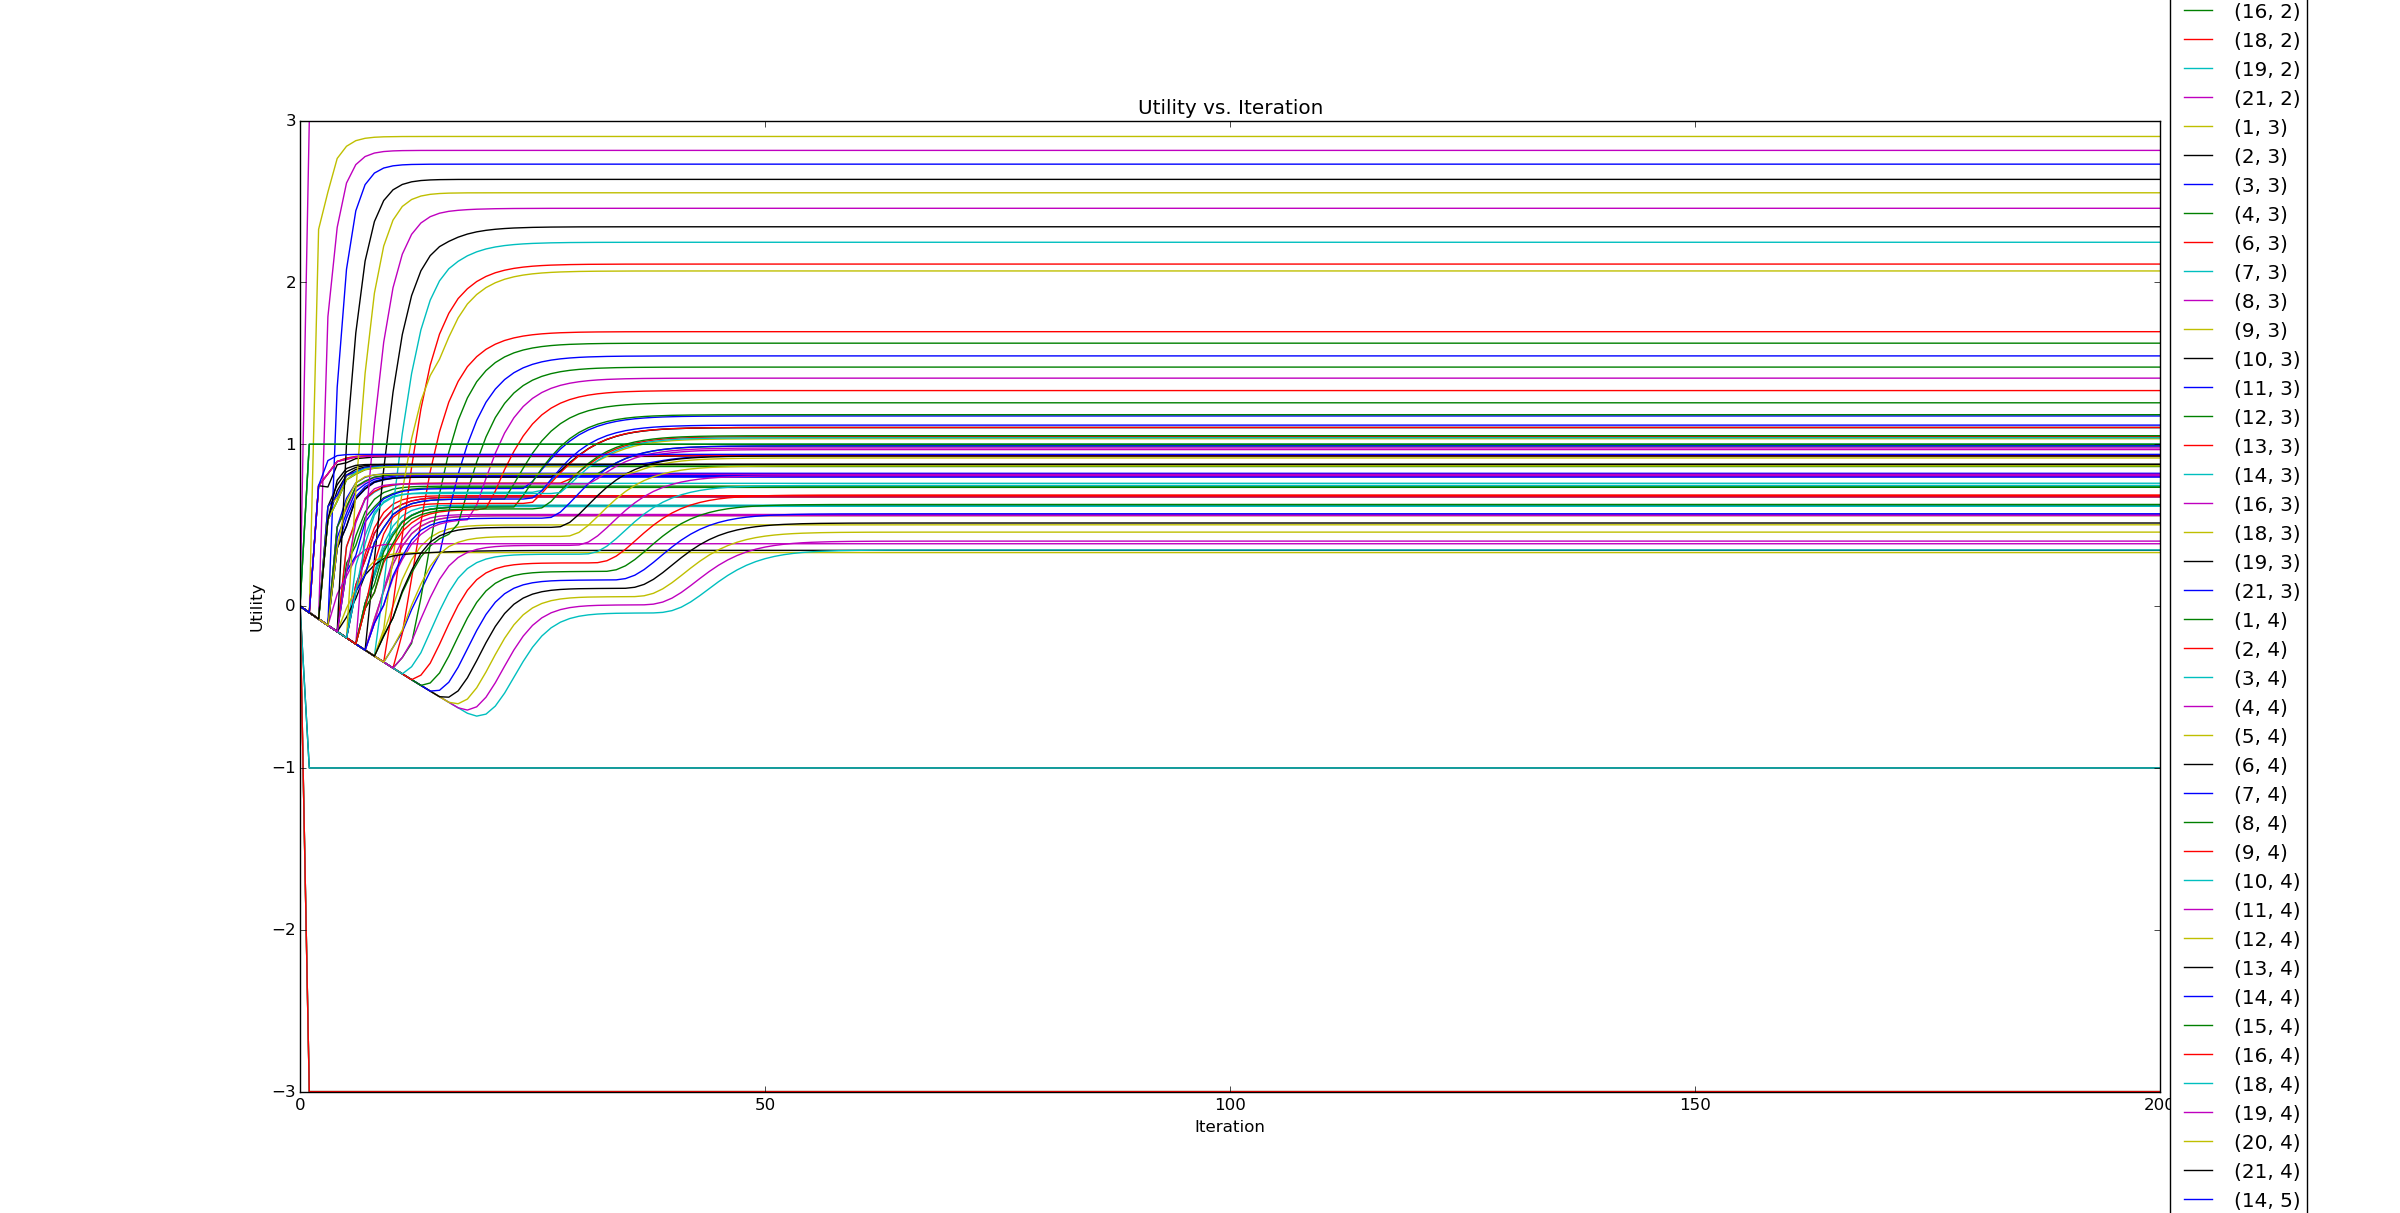
\includegraphics[width=\linewidth]{graphics/term_11ec_util_iters.png}
  \caption{Terminal rewards: utility estimates vs number of iterations}
\end{figure}

\subsubsection{Non-terminal rewards value iteration}
\begin{figure}[H]
  \centering
  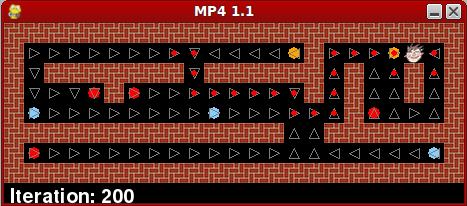
\includegraphics[width=0.5\linewidth]{graphics/inf_11ec_opti_policy.png}
  \caption{Non-terminal rewards: optimal policy (ended on a +3 reward state with policy arrow oscillating up and down)}
\end{figure}

%% \paragraph{Utilities}
%% \begin{tabular}{|l|l|l|l|l|l|l|l|l|l|l|l|l|l|l|l|l|l|l|l|l|l|l|}
%% 0 & 0 & 0 & 0 & 0 & 0 & 0 & 0 & 0 & 0 & 0 & 0 & 0 & 0 & 0 & 0 & 0 & 0 & 0 & 0 & 0 & 0 & 0
%% 0 & 130.4733776739696 & 132.39206575533063 & 134.49241749201903 & 136.61928882134237 & 138.773014586642 & 140.9539338590793 & 143.16238999101708 & 145.3987306700753 & 147.66330797386908 & 145.3987306700753 & 143.16238999101708 & 140.9539338590793 & 138.773014586642 & 135.42228134004557 & 0 & 181.2261359018459 & 184.2784627370733 & 187.03394574878374 & 190.13080974864886 & 194.5594152428118 & 191.36329417467212 & 0
%% 0 & 131.73288003968327 & 0 & 0 & 0 & 0 & 0 & 0 & 0 & 150.52262275138642 & 0 & 0 & 0 & 0 & 0 & 0 & 178.54306947176815 & 0 & 184.58122946089054 & 187.03394574878374 & 0 & 188.55382926238954 & 0
%% 0 & 133.8249087244064 & 134.91268650815806 & 136.79825862363907 & 136.00398606871406 & 0 & 143.07283129609513 & 148.55624882302814 & 150.71023153544957 & 152.8518956622675 & 155.26186701436612 & 157.38450673176018 & 159.62810628860387 & 161.854780123838 & 164.0524296402715 & 0 & 175.89345773533225 & 0 & 182.09612019179866 & 184.03867149181008 & 0 & 185.77939508467404 & 0
%% 0 & 135.80737968975566 & 136.88553163466858 & 139.28922469246544 & 141.78803252787247 & 144.73002601605344 & 146.9861600792662 & 149.7599467815774 & 152.23005219018356 & 154.77086113541642 & 157.39364410397684 & 158.7630131580364 & 161.36864470561923 & 164.0524296402715 & 166.82723963576842 & 169.98359839665892 & 172.91502425055322 & 0 & 176.25836861064863 & 180.6890994363014 & 180.00455596199538 & 182.70607550432348 & 0
%% 0 & 0 & 0 & 0 & 0 & 0 & 0 & 0 & 0 & 0 & 0 & 0 & 0 & 0 & 164.63229382961165 & 167.13212996823697 & 0 & 0 & 0 & 0 & 0 & 0 & 0
%% 0 & 128.9004520247075 & 134.6940914668173 & 136.82350918471138 & 138.97981348995262 & 141.16334385965393 & 143.37444405725554 & 145.61346218664502 & 147.88075074696116 & 150.1766666880894 & 152.50157146685805 & 154.8558311039445 & 157.2398162414993 & 159.65390220149794 & 162.0984690448298 & 164.0758983003331 & 161.60667523187024 & 159.1682404809692 & 156.76021015339614 & 154.38220514162816 & 152.03385106516905 & 151.0115363163466 & 0
%% [0 & 0 & 0 & 0 & 0 & 0 & 0 & 0 & 0 & 0 & 0 & 0 & 0 & 0 & 0 & 0 & 0 & 0 & 0 & 0 & 0 & 0 & 0
%% \end{tabular}

\begin{figure}[H]
  \centering
  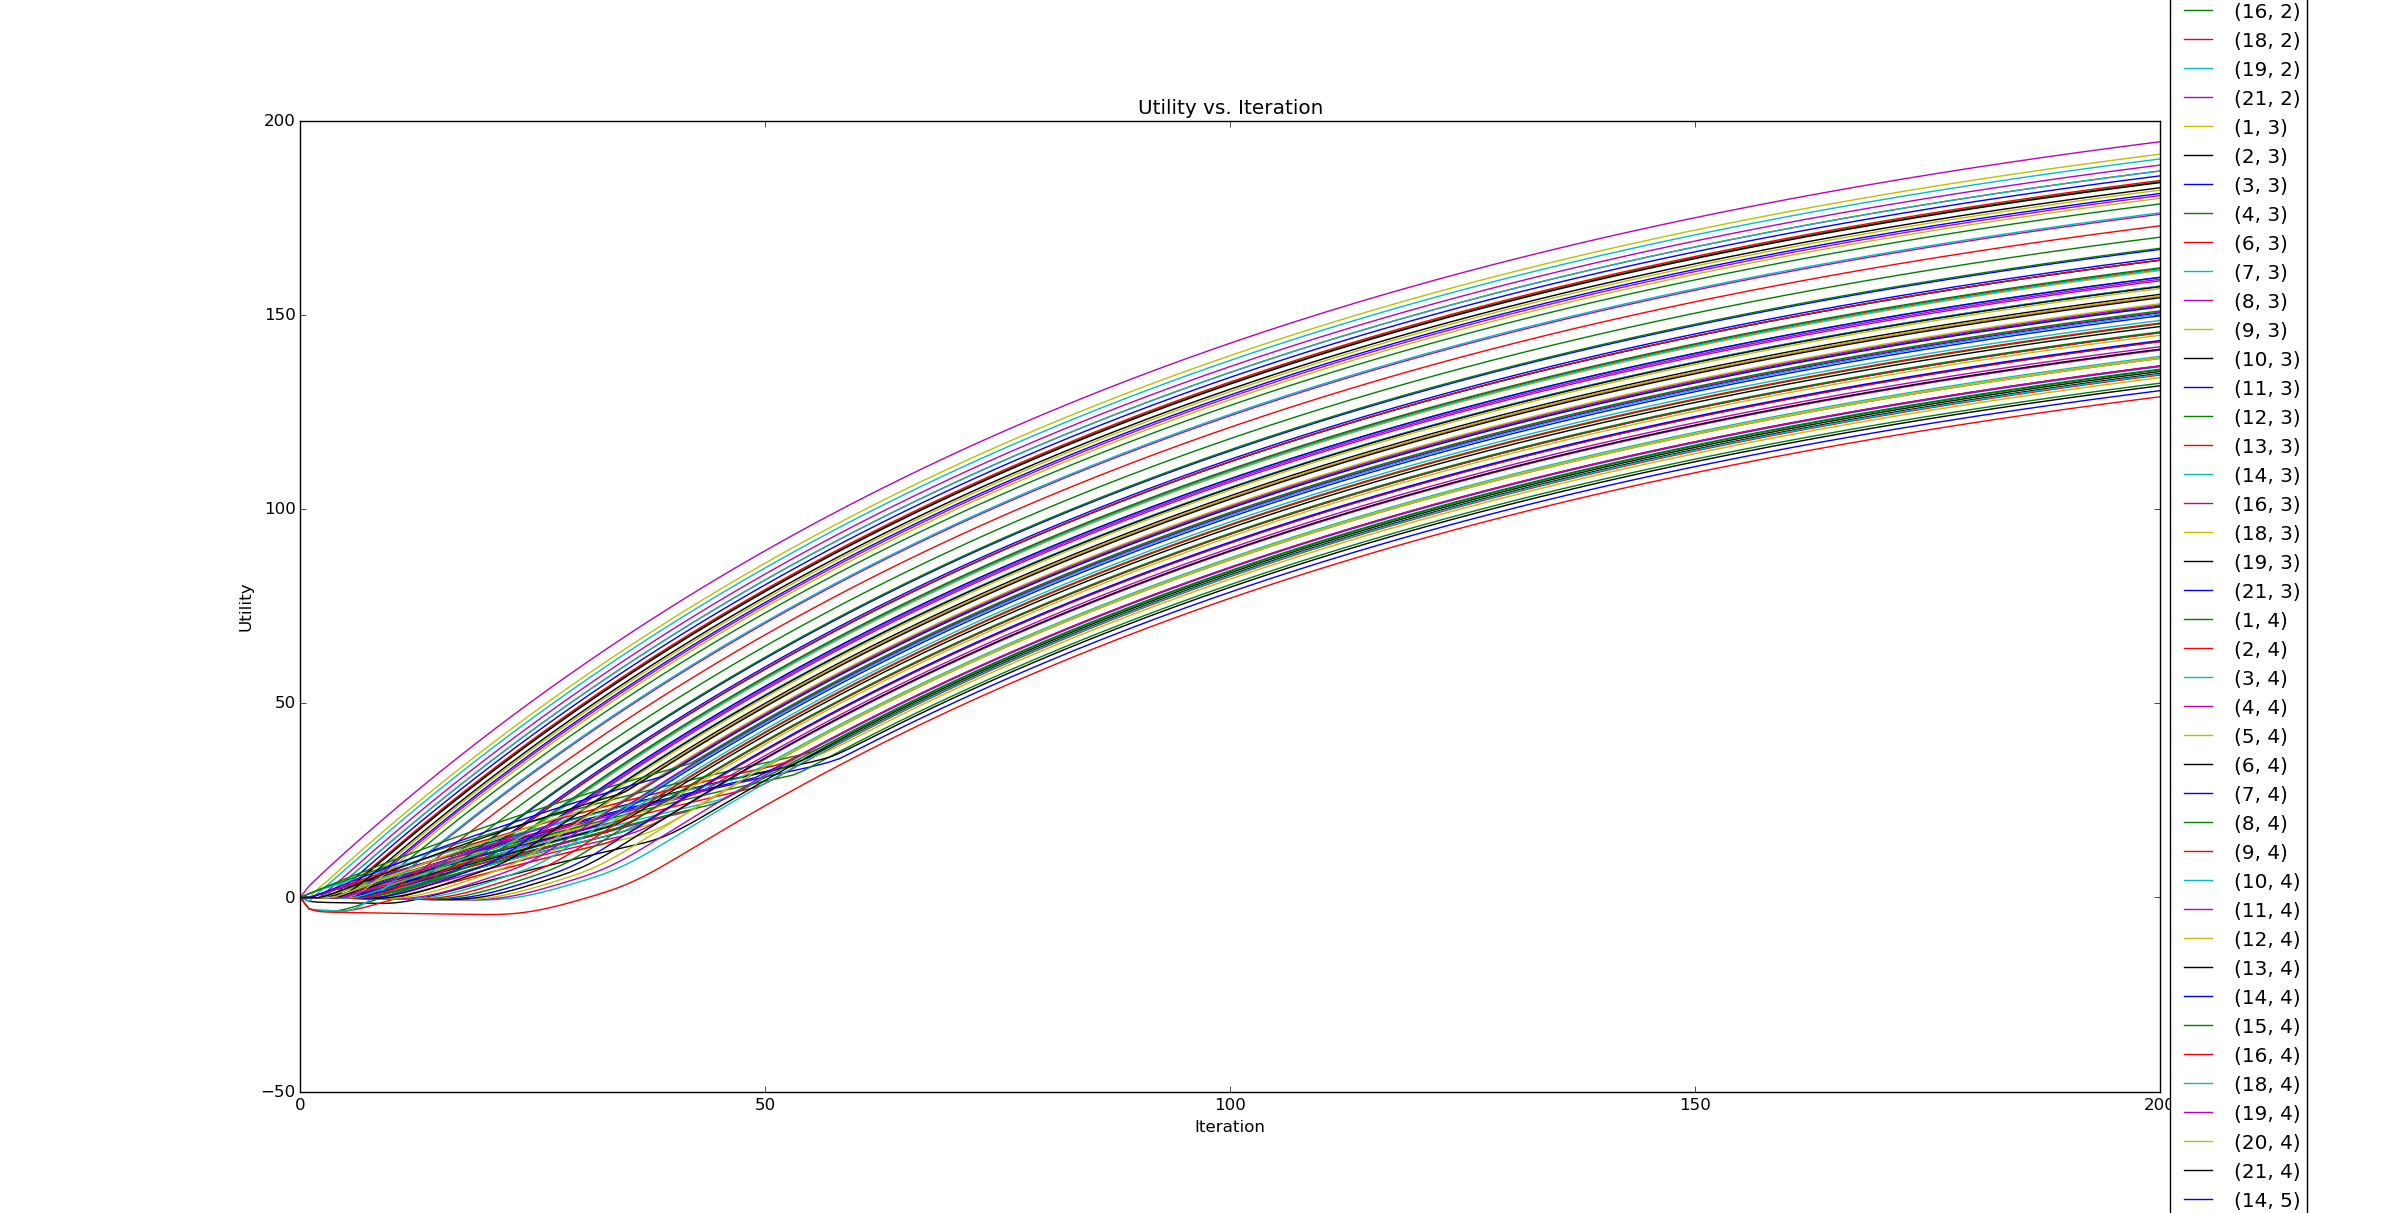
\includegraphics[width=\linewidth]{graphics/inf_11ec_util_iters.png}
  \caption{Non-terminal rewards: utility estimates vs number of iterations}
\end{figure}

\subsubsection{TD Q-learning}
\begin{figure}[H]
  \centering
  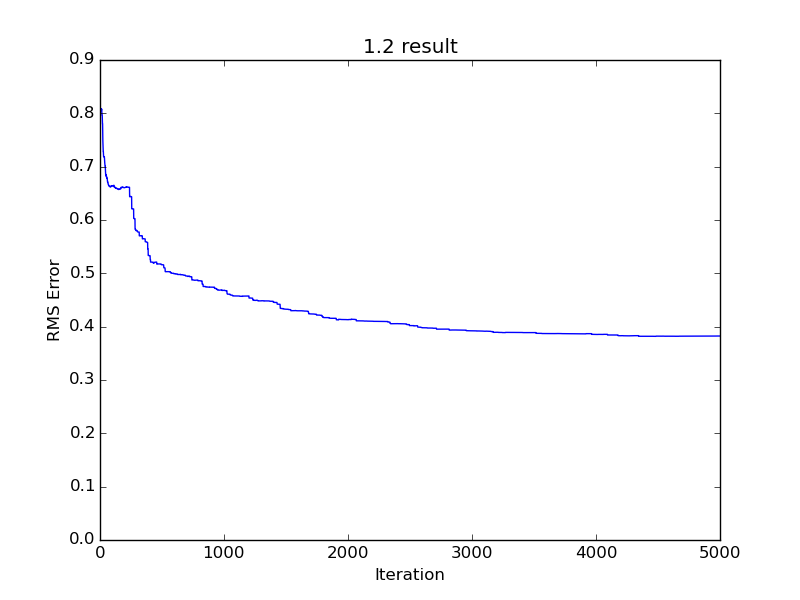
\includegraphics[width=0.5\linewidth]{graphics/rmse_plot_12ec.png}
  \caption{RMS error vs number of iterations}
\end{figure}
The RMS error is rather high throughout the plot since the pacman oscillates up and down at the end coordinate; since there are wall above and below it, the pacman cannot move, and the end result is not affected, but the RMS error is affected.

\subsection{Part 1.3: Pizza Delivery}
%% \begin{itemize}
%%   \item \Fix{Discuss implementation and parameter settings.}
%%   \item \Fix{Show final policy in the form of four maps corresponding to all possible ingredient/pizza combinations.}
%% \end{itemize}

We implemented Q-learning with the following parameters:
\begin{itemize}
  \item Number of iterations: 10000. We cut off the number of steps at 100 since the states are non-terminal and could lead to any number of steps.
  \item Gamma: 0.99
  \item Learning rate decay: $\frac{200}{199+t}$, where $t$ is the trial number.
  \item Exploration function: if the number of visited places is less than 300, then try a random action. Otherwise, follow the standard exploration function on slide 21 of lecture 17 (Reinforcement learning).
\end{itemize}

In our Q-learning implementation, each coordinate in the map is associated with a single policy (direction) and sixteen different utility values derived for each combination of the four directions and four states (of ingredients/pizza). Therefore, we created the data structures utility\_ ra = max{value[height][width][state]} and value\_ ra[height][width][state][action]. The latter holds the values at each coordinate (height, width), similar to the figure on slide 22 of lecture 17 (Reinforcement learning), but instead of just holding values for four directions, it must hold values for each combination of the four directions and states, leading to 16 values per coordinate. The utility at the coordinate is the maximum of these 16 values.

\begin{figure}[H]
  \centering
  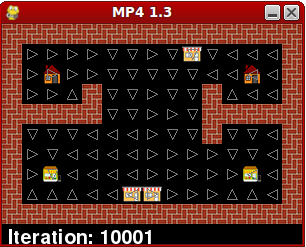
\includegraphics[width=0.4\linewidth]{graphics/state0_13.png}
  \caption{State: No ingredients, no pizza}
\end{figure}

\begin{figure}[H]
  \centering
  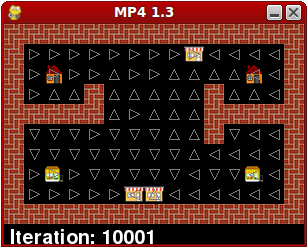
\includegraphics[width=0.4\linewidth]{graphics/state1_13.png}
  \caption{State: Ingredients, but no pizza}
\end{figure}

\begin{figure}[H]
  \centering
  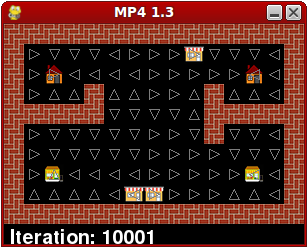
\includegraphics[width=0.4\linewidth]{graphics/state2_13.png}
  \caption{State: Pizza, but no ingredients}
\end{figure}

\begin{figure}[H]
  \centering
  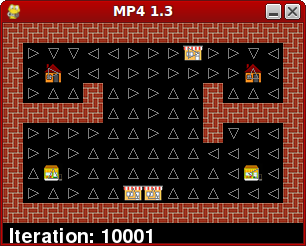
\includegraphics[width=0.4\linewidth]{graphics/state3_13.png}
  \caption{State: Ingredients, pizza}
\end{figure}

These maps depicting the resulting policies for each state make sense since, for example, in the state when we have neither ingredients nor pizza, the policy arrows direct us away from the students and pizza shops, and towards the grocery stores to pick up groceries to make pizzas with. When we have groceries but no pizza, the policy arrows direct us towards the pizza shops, so we can make the pizzas before delivery; this makes sense since we cannot go pick up more ingredients since we can only carry one pizza's worth of them, and we don't have any pizzas to deliver. When we have just pizzas, the policy arrows direct us towards either students, to deliver the pizzas to, or to grocery stores to pick up ingredients for more pizzas with. Finally, if we have both pizzas and ingredients, the policies direct us towards the students so that we can deliver the pizzas in preparation for make more pizzas to free up our ingredients.

\subsection{Extra credit: 1.3}
We added extra rules to account for and penalize the time spent buying ingredients, cooking the pizza, and handing off the pizza to the student. We also added a rule to reward delivery tips based on Manhattan distance, where $tips = 0.1 * \textit{last visited pizza chain} * destination$.

\begin{figure}[H]
  \centering
  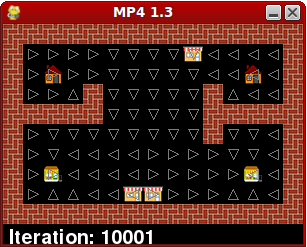
\includegraphics[width=0.4\linewidth]{graphics/state0_13ec.png}
  \caption{State: No ingredients, no pizza}
\end{figure}

\begin{figure}[H]
  \centering
  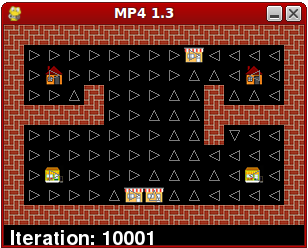
\includegraphics[width=0.4\linewidth]{graphics/state1_13ec.png}
  \caption{State: Ingredients, but no pizza}
\end{figure}

\begin{figure}[H]
  \centering
  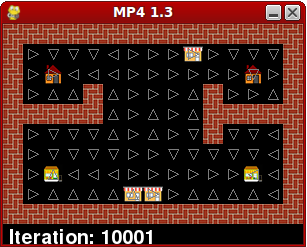
\includegraphics[width=0.4\linewidth]{graphics/state2_13ec.png}
  \caption{State: Pizza, but no ingredients}
\end{figure}

\begin{figure}[H]
  \centering
  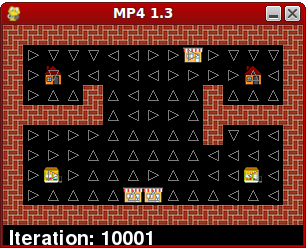
\includegraphics[width=0.4\linewidth]{graphics/state3_13ec.png}
  \caption{State: Ingredients, pizza}
\end{figure}

These maps depicting the resulting policies for each state make sense based on the new rules. When we have neither ingredients nor pizza, the policies direct us towards the grocery stores so that we can buy some to make and sell pizza with. When we have just ingredients, the policies direct us to cook at upper pizza shop, rather than a pizza shop closer to the students and points us away from the farther shops since this reduces the time spent delivering. When we have just pizza, the policies direct us towards either the students, so that we can sell the pizza, or the grocery stores, so that we can stock up on more ingredients with which to cook more pizza. When we have both ingredients and pizza, the policies direct away from the groceries, since we can't hold any more ingredients, and away from the pizza shops as well since we have pizzas to deliver; the policies point us towards the students so that we can sell the pizzas. Compared with the fact that the policies tend to direct us to sell the pizza to the upper right student with the original rules, the policies are well balanced with new rules.